\section{Cross-Condition Validation and Diagnostics}
\label{sec:cross_condition}

A 0.49~pp gain on a single development set is not a transferability claim. Here the same
recipe — $\tau=10$, CER loss, RoBERTa PLL posterior — runs without modification across two
Zipformer architectures, three domains, and four noise levels, with the held-out LibriSpeech
test-other split evaluated for the first time. The §5 MBR result on dev-other provides the
baseline; four diagnostic experiments then establish where the approach reaches its ceiling.



\subsection{Cross-Condition Results}

\begin{figure*}[t]
  \centering
  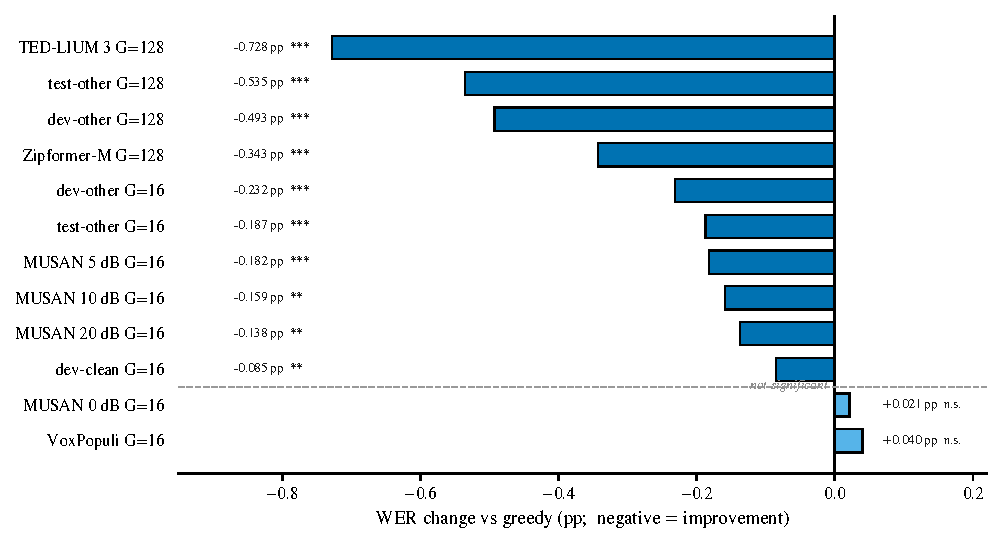
\includegraphics[width=\textwidth]{figures/fig7_cross_condition.pdf}
  \caption{WER change (MBR-CER+PLL vs greedy, pp) across all evaluation conditions. Sorted by improvement magnitude; light blue: not significant. Significance from paired bootstrap ($B=10{,}000$, seed 42): $*p<0.05$, $**p<0.01$, $***p<0.001$. VoxPopuli: coverage-bottlenecked (91.5\% of utterances already greedy-optimal, oracle gap only 0.31\,pp). MUSAN 0\,dB: candidate quality degrades under extreme noise.}
  \label{fig:cross-condition}
\end{figure*}

Table~\ref{tab:cross-condition} reports results for every condition evaluated in this work; Figure~\ref{fig:cross-condition} visualizes gap-closure percentages across conditions. The
configuration was fixed throughout: $\tau$=10, CER loss, RoBERTa PLL posterior, paired bootstrap
$B$=10\,000, seed=42, all comparisons against greedy decoding. No hyperparameter was adjusted after
the dev-other experiments described in §5.

\begin{table*}[t]
\centering
\caption{Cross-condition summary: MBR-CER\,+\,RoBERTa PLL ($\tau$=10) vs greedy decoding.
$\Delta$ = MBR$\,-\,$greedy (pp). Gap closure = $-\Delta\,/\,(\text{greedy}-\text{oracle})$.
Significance: paired bootstrap, $B$=10\,000, seed=42, vs greedy. n.s.\ = $p>0.05$.
VoxPopuli WERs are punct-stripped (raw: greedy 21.93\%, MBR 21.97\%); see Appendix~B.3.
See Appendix~A.1 for 95\% bootstrap confidence intervals on all conditions.
MUSAN: LibriSpeech dev-other utterances with additive MUSAN noise
\cite{snyder2015musan}; $G$=16. All TL3/VoxPopuli/MUSAN runs use nbest\_scale=1.0.}
\label{tab:cross-condition}
\begin{tabular}{llrrrrrr}
\hline
Condition & $G$ & Greedy (\%) & Oracle (\%) & MBR+PLL (\%) & $\Delta$ (pp) & $p$ & Gap cl.\ (\%) \\
\hline
\multicolumn{8}{l}{\textit{In-domain (LibriSpeech)}} \\
dev-clean  & 16  & 2.37 & 1.54 & 2.28 & $-$0.09 & 0.008      & 10.3 \\
dev-other  & 16  & 6.02 & 4.44 & 5.79 & $-$0.23 & $<$0.0001  & 14.7 \\
dev-other  & 128 & 6.02 & 3.53 & 5.53 & $-$0.49 & $<$0.0001  & 19.8 \\
test-other & 16  & 5.96 & 4.41 & 5.77 & $-$0.19 & 0.0003     & 12.1 \\
test-other & 128 & 5.96 & 3.37 & 5.42 & $-$0.54 & $<$0.0001  & 20.7 \\
\hline
\multicolumn{8}{l}{\textit{Cross-architecture (Zipformer-M, 65M params, LibriSpeech dev-other)}} \\
Zipformer-M & 16  & 4.78 & 3.44 & 4.56 & $-$0.22 & $<$0.0001 & 16.5 \\
Zipformer-M & 128 & 4.78 & 2.73 & 4.43 & $-$0.34 & $<$0.0001 & 16.8 \\
\hline
\multicolumn{8}{l}{\textit{Out-of-domain}} \\
TED-LIUM 3 & 16  & 11.30 & 9.16 & 10.97 & $-$0.33 & $<$0.0001 & 15.6 \\
TED-LIUM 3 & 128 & 11.30 & 7.51 & 10.57 & $-$0.73 & $<$0.0001 & 19.2 \\
VoxPopuli  & 128 & 18.29 & 17.97 & 18.33 & $+$0.04 & n.s.      & ---  \\
\hline
\multicolumn{8}{l}{\textit{Noise (MUSAN additive, $G$=16)}} \\
MUSAN 20 dB & 16 & 6.62 & 4.89 & 6.38 & $-$0.24 & 0.006  & 13.9 \\
MUSAN 10 dB & 16 & 8.04 & 6.26 & 7.80 & $-$0.24 & 0.003  & 13.5 \\
MUSAN 5 dB  & 16 & 11.10 & 9.06 & 10.84 & $-$0.27 & 0.001 & 13.0 \\
MUSAN 0 dB  & 16 & 17.88 & 15.57 & 17.64 & $-$0.23 & 0.646 & --- \\
\hline
\end{tabular}
\end{table*}

\textbf{In-domain generalization.} On LibriSpeech dev-clean, where greedy WER is already 2.37\%,
MBR-CER+PLL at $G$=16 reached 2.28\% ($\Delta$=$-$0.085~pp, $p$=0.008, 95\%\ CI
[$-$0.156, $-$0.016]~pp). Only 13.9\% of dev-clean utterances had any candidate
better than greedy in the $G$=16 candidate set, versus 23.2\% on dev-other. The smaller
recoverable fraction directly explains the smaller absolute gain. Proportional reductions are
consistent across the two splits: 3.6\% relative on dev-clean and 3.9\% relative on dev-other at
$G$=16. Spearman $\rho$ for RoBERTa PLL was in fact stronger on dev-clean ($-$0.496) than on
dev-other ($-$0.484), confirming that cleaner audio produces more reliable PLL rankings. The
smaller absolute gain therefore reflects a data ceiling, not a method degradation.

The held-out test-other evaluation is the strictest test in this work. No hyperparameter was
adjusted after dev-other experiments; $\tau$=10 and CER loss were fixed. At the practical beam
size $G$=16, MBR-CER+PLL reached 5.77\% (greedy 5.96\%, $\Delta$=$-$0.187~pp, $p$=0.0003,
95\%\ CI [$-$0.288, $-$0.086]~pp), closing 12.1\% of the $G$=16 oracle gap. At $G$=128 the gain
widened to 5.42\% ($\Delta$=$-$0.535~pp, $p<0.0001$, 95\%\ CI [$-$0.629, $-$0.441]~pp), a 9.0\%
relative reduction closing 20.7\% of the oracle gap.
The gain strengthened on test-other relative to
dev-other ($-$0.535~pp vs $-$0.493~pp at $G$=128), a pattern inconsistent with dev-other overfitting. Seven of ten configurations tested on test-other reached statistical
significance at $G$=128, compared with six of ten on dev-other.

\textbf{Cross-architecture transfer.} To test whether the recipe depends on the Zipformer-S
architecture, the same settings were applied without modification to Zipformer-M, a 65M-parameter
variant with a deeper encoder (layer counts 2--2--3--4--3--2, dimensions 192--512), which is
approximately three times the parameter count of Zipformer-S. On
dev-other at $G$=16, Zipformer-M achieved 4.56\% (greedy 4.78\%, $\Delta$=$-$0.220~pp,
$p<0.0001$), closing 16.5\% of the oracle gap. At $G$=128, the gain widened to $-$0.344~pp
($p<0.0001$, gap closure 16.8\%), replicating the beam-scaling behavior of Zipformer-S documented
in §5.3.

The ranking diagnostics also replicated. The Spearman $\rho$ values were near-identical across architectures: CTC
$\rho$=$-$0.350 (Zipformer-S: $-$0.347) and PLL $\rho$=$-$0.482 (Zipformer-S: $-$0.484) at
$G$=16. At $G$=128, the CTC--PLL divergence documented in §5.3 reappeared:
CTC $\rho$ fell to $-$0.288 while PLL $\rho$ held at $-$0.459. The ranking
degradation with beam size is a property of CTC lattice sampling, not of the specific
architecture. MBR benefits from PLL posteriors because PLL ranking quality is insensitive to
blank-path proliferation at large $G$; this property holds in the 65M-parameter model as fully
as in the 22M-parameter one.

\textbf{Out-of-domain transfer.} Two out-of-domain datasets were evaluated without any
domain-specific adjustment. TED-LIUM~3 (1155 utterances of parliamentary and lecture speech from
public TED recordings \cite{hernandez2018tedlium3}) shares no acoustic domain, speaker style, or
vocabulary with LibriSpeech. The BPE-500 tokenizer cannot represent many TED proper nouns,
raising deletion rates to 19\% (vs 13\% on dev-other) and insertion rates to 18\%. Despite this,
the oracle gap at $G$=128 was 3.79~pp (greedy 11.30\%, oracle 7.51\%), wider in absolute terms
than on dev-other (2.49~pp), likely because systematic function-word and morpheme-level errors populate
the N-best with alternatives that the LM can rank. 60.8\% of TL3 utterances had at least one
candidate better than greedy at $G$=128. MBR-CER+PLL at $G$=128 reached 10.57\%
($\Delta$=$-$0.728~pp, $p<0.0001$, 95\%\ CI [$-$0.883, $-$0.581]~pp), closing 19.2\% of the
oracle gap. At $G$=16, the gain was $-$0.334~pp ($p<0.0001$, gap closure
15.6\%). The pattern aligns with §5.2: cross-domain errors
introduce vocabulary-level variation that a bidirectional masked LM can disambiguate across
candidates, even when absolute WER is nearly double that of dev-other.

VoxPopuli (1842 utterances of European Parliament speech \cite{wang2021voxpopuli}) produced a
qualitatively different outcome. After punctuation stripping to correct for BPE-500's inability to
produce punctuation tokens (raw greedy 21.93\% $\to$ corrected 18.29\%; see Appendix~B.3), the
oracle gap at $G$=128 was 0.31~pp, approximately 8 times smaller than on dev-other. Only 8.5\%
of utterances had any candidate better than greedy in a 128-candidate set; MBR selected the oracle in most cases when one was available, but that population constitutes only 157 of 1842
utterances. MBR-CER+PLL at $G$=128 produced 18.33\%
($\Delta$=$+$0.04~pp) — marginally and non-significantly worse than greedy. Wider beams do not
open this gap: beam sensitivity tests at output\_beam $\in$ \{8, 10, 12, 15, 20\} showed oracle
WER saturating at beam=10 and remaining identical at beam=12--20; the original beam=8 setting was
not the binding constraint.

This result confirms the boundary condition established by the Spearman $\rho$ divergence analysis
in §5.3. The CTC posterior on European Parliament speech concentrates around a wrong greedy
output rather than spreading into diverse, reference-aligned alternatives. The N-best is
orthographically diverse (9.33~pp WER spread per utterance at $G$=128) but 91.5\% of that
diversity is worse than greedy. When CTC ranking quality collapses under distribution shift — as the $\rho$
degradation from $-$0.347 (LibriSpeech) to $-$0.304 (TL3) and the coverage collapse on
VoxPopuli jointly illustrate — PLL has nothing useful to rerank.

\textbf{Noise robustness.} MUSAN additive noise \cite{snyder2015musan} was applied to LibriSpeech
dev-other utterances at four SNR levels. N-best lists were generated at $G$=16 with
nbest\_scale=1.0, and the same canonical MBR-CER+PLL $\tau$=10 configuration was applied
unchanged. At SNR $\geq$ 5~dB, the gain was statistically
significant: 20~dB ($\Delta$=$-$0.24~pp, $p$=0.006), 10~dB ($\Delta$=$-$0.24~pp, $p$=0.003),
5~dB ($\Delta$=$-$0.27~pp, $p$=0.001). Gap closure was stable at 13.0--13.9\% across these three
conditions. The proportional gain is slightly below the clean-speech value of 14.7\% at $G$=16,
consistent with the Spearman $\rho$ degradation from $-$0.347 (clean) to $-$0.306 at 0~dB: CTC
ranking quality decreases under noise, but PLL ranking remains informative enough to produce
significant improvements at moderate SNR.

At 0~dB, the gain is not statistically significant ($\Delta$=$-$0.24~pp, $p$=0.646). This is not
a coverage error: the oracle gap at $G$=16 is 2.31~pp at 0~dB and 33.3\% of utterances are
recoverable. At 0\,dB, both candidate quality and candidate diversity are degraded. A controlled intervention---widening the beam ($\text{beam}=20$) or flattening the sampling distribution (\texttt{nbest\_scale=0.5})---increased the unique-candidate count from 12.8 to 15.3 but destroyed oracle quality (17.73\% $\to$ 19.37\%) without restoring MBR gains. The binding constraint is candidate quality, not candidate variety: forced diversity at the cost of quality collapses MBR rather than recovering it. The Spearman $\rho$ degradation under noise (§5.3) remains valid as a correlational observation.



\subsection{Diagnostics: Selection vs Coverage and MBR Exhaustion}

Four diagnostics establish the ceiling of the decode-time approach.

\textbf{Selection versus coverage.} The 2.49~pp oracle gap on LibriSpeech dev-other at $G$=128
decomposes into two components: coverage error (oracle absent from the candidate set) and
selection error (oracle present but not selected by MBR). A decomposition analysis on all 2864 dev-other utterances across $G \in \{4, 8, 16, 32, 64, 128\}$ measured this breakdown. At $G$=128, the candidate set was 89\% unique (mean 113.7 of 128 candidates
distinct); 33.7\% of utterances had an oracle that beat greedy. MBR-CER+PLL selected the oracle
in 137 of 964 recoverable utterances (14.2\%). In recoverable utterances, the oracle's median
rank in the MBR risk ordering was 6 (mean rank 20.4); 15.4\% of oracles ranked below position
50. In this selection-vs-coverage decomposition, MBR recovered 0.47~pp of the 2.49~pp total
gap --- a per-utterance selection quantity, distinct from the corpus-level $-$0.49~pp headline
gain. The residual was 2.01~pp, which is 81\% of the recoverable gap.

The selection error implies that the MBR scoring surface is too flat to consistently distinguish
the oracle from close alternatives. In 83\% of recoverable utterances, MBR selected a hypothesis
within one word edit of the oracle — nearby but not correct. This diagnostic establishes that the
bottleneck is not in the coverage of the candidate set but in the precision of the scoring
function. Expanding the beam beyond $G$=128 improves oracle WER (the coverage axis) at
roughly 0.28~pp per doubling, but leaves the 2.01~pp selection gap untouched.

\textbf{MBR hyperparameter sweep.} A systematic search over 63 configurations on the $G$=128
candidate set — temperature $\tau \in \{0.5, 1, 2, 5, 10, 20, 50, 100, \infty\}$, loss
$\in \{$CER, WER, BPE-edit, neg-BLEU$\}$, posterior $\in \{$PLL, CTC, GPT-2, product-of-experts$\}$,
and two-stage filtering at $K \in \{3, 5, 10, 20\}$ — identified MBR-WER+PLL $\tau$=10 as the
sweep optimum: 5.46\% WER. The improvement over the CER-loss baseline
(5.53\%) is 0.07~pp and statistically significant ($p$=0.002, 95\%\ CI [$-$0.12,
$-$0.02]~pp). The residual gap after tuning is 1.93~pp versus 2.01~pp before. The WER-loss
result is excluded from all primary comparisons because WER loss with WER evaluation is
circular (§5.2); CER loss (5.53\%) is the fair result throughout this work.

Adding GPT-2 to the PLL posterior in any weight configuration hurt WER. GPT-2 Spearman
$\rho$=$-$0.361 at $G$=128 is substantially weaker than PLL $\rho$=$-$0.461; adding a noisier
scorer to a stronger one dilutes the posterior and shifts the MBR risk surface away from the PLL
optimum. The temperature $\tau$=10, confirmed as optimal by the full sweep, validates the
§5.4 calibration result independently. The MBR framework as implemented — pairwise distance
matrix, log-linear posterior, fixed loss — appears near-exhausted within the tested configuration space. No available combination of
signals closes more than 0.07~pp of the 2.01~pp selection gap.

\textbf{DistilBERT MWER reranker.} A DistilBERT discriminative reranker \cite{sanh2019distilbert} was trained with MWER loss on LibriSpeech train-clean-100 (28,539 utterances $\times$ 16 candidates) and evaluated on dev-other at $G$=128. The optimal mixing weight was $\beta$=0 across all configurations — the system discarded the reranker entirely ($p$=1.000 for all comparisons vs.\ MBR-CER+PLL baseline). This parallels §4's finding: train-clean-100 lacks sufficient MWER reward signal (greedy-oracle gap 0.007~pp) to train a discriminative reranker that adds value beyond PLL. The MWER reranker is the decode-time instantiation of the same boundary condition that §4.5 identified for training-time RL. See Appendix~C.2 for training convergence details and mixing-weight sweep.

\textbf{Ensemble LM.} An ensemble posterior combining RoBERTa PLL and GPT-2 log-likelihood via $s = \beta\,\text{PLL} + (1-\beta)\,\text{GPT-2 LL}$ was evaluated by sweeping $\beta$ over seven
values at three temperatures on the $G$=128 candidate set. The best ensemble
configuration ($\beta$=0.8, $\tau$=7) produced 5.514\%, a $-$0.016~pp change versus RoBERTa
alone that did not reach statistical significance ($p$=0.305, 95\%\ CI [$-$0.063,
$+$0.031]~pp). Pure GPT-2 posterior ($\beta$=0) produced 5.694\% — substantially worse than PLL
alone. The tiebreaker variant (MBR top-5 then GPT-2 argmax) produced 6.350\%, worse than greedy.
GPT-2 Spearman $\rho$=$-$0.361 at $G$=128 is weaker than PLL $\rho$=$-$0.461; adding a
weaker scorer at any weight introduces noise. The information bottleneck established in §5.1
extends to the external-LM stage: the linguistic information accessible to text-only scoring on
this candidate set is fully captured by RoBERTa PLL, and a second LM cannot expand the channel.



Eleven of thirteen conditions showed significant improvement; the two non-significant results---VoxPopuli (coverage-bottlenecked) and MUSAN at 0\,dB (candidate quality degraded)---align with conditions where the Spearman $\rho$ divergence analysis in §5.3 predicted reduced MBR efficacy.

After Holm-Bonferroni correction for the 13 simultaneous tests in
Table~\ref{tab:master-full}, all 11 conditions originally reported
as significant remain so (worst adjusted $p = 0.019$, dev-clean $G=16$).
Benjamini-Hochberg FDR control at $q=0.05$ produces the same set of
rejections. VoxPopuli ($\Delta = +0.04$\,pp) and MUSAN 0\,dB (raw $p = 0.646$) are non-significant before
and after correction; the two failures are interpreted substantively
(\S\ref{sec:cross_condition}) rather than as multiple-testing artifacts.
